\documentclass[a4paper]{article}

\usepackage{fullpage}
\usepackage[utf8]{inputenc}
\usepackage[english]{babel}
\usepackage{graphicx}

\title{Operating Systems\\Simple Versioning File System}
\author{Louis Lettry, Nicolas Sanglard, Damien Firmenich}
\date{}	

\begin{document}
\maketitle

\section{Introduction}
The aim of the project is to implement a file system which we can use to manipulate standard files, in addition to the already existing file system. The FUSE library is well suited for this job, because it allows us to manipulate files directly in user space, thus avoiding any kernel failures. FUSE works by setting callbacks for every file manipulation, and sets those callbacks on a mount point defined when launching the file system.

The file system we had to implement is a simple versioning file system, which keeps copy of modified files during a precise number of minutes.

\section{SVFS}
The implementation of the Simple Versioning File System was done using 2-level linked lists. The first list contains a structure for files in the file system, and each file structure contains another list used to store a structure for each backup of the file. The schema of the list structure is shown in Figure \ref{fig:schema}, where the fields in each struct are depicted.

In each callback, we called certain functions to manipulate the lists, especially when the user writes to the file, deletes it, or renames it.

Then, we need to take care of the created backups so that they are not kept longer than a certain amount of time. Thus we implemented a garbage collector which scans the structure every $\Delta_t$ and choose which backups have expired, and deletes them. The expiring time is modified depending on the frequency of modification of the file, extending it when is frequently used.

\begin{figure}[h!]
	\centering
	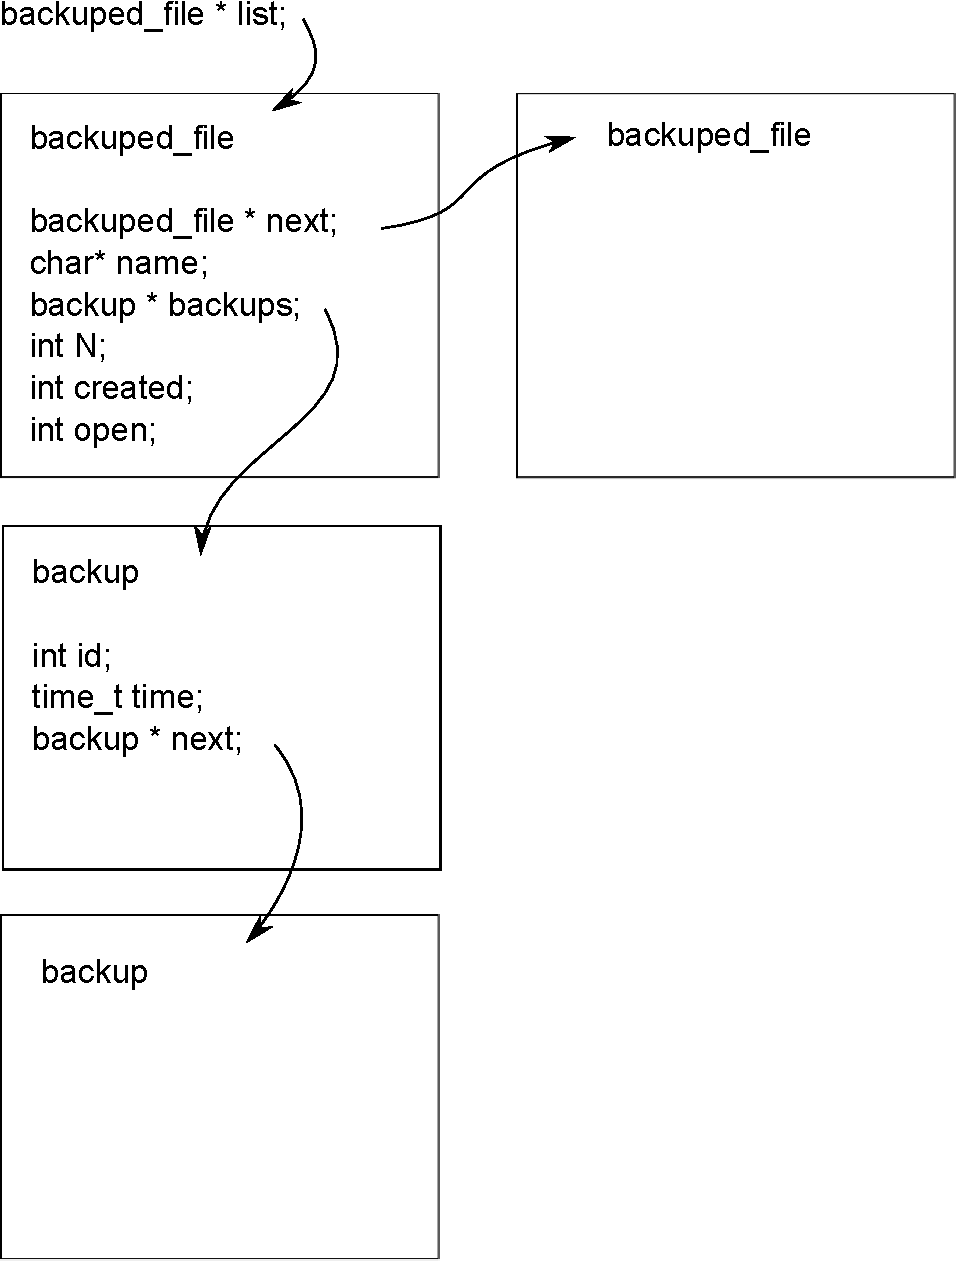
\includegraphics[width=0.7\columnwidth]{schema.pdf}
	\caption{List structure \label{fig:schema}}
\end{figure}

\section{Conclusion}
The main point we can retain from our experience is that creating a whole new file system is really easy with FUSE because little knowledge of the internal structure is needed. The implementation is also safe because it runs in user space so it does not affect the kernel directly.

\end{document}
